\documentclass{beamer}
\mode<presentation> {
\usepackage{color}
\definecolor{bottomcolour}{rgb}{0.21,0.11,0.21}
\definecolor{middlecolour}{rgb}{0.21,0.11,0.21}
\setbeamercolor{structure}{fg=white}
\setbeamertemplate{frametitle}[default]%[center]
\setbeamercolor{normal text}{bg=black, fg=white}
\setbeamertemplate{background canvas}[vertical shading]
[bottom=bottomcolour, middle=middlecolour, top=black]
\setbeamertemplate{items}[circle]
\setbeamertemplate{navigation symbols}{} %no nav symbols
\setbeamercolor{block title}{use=structure,fg=white,bg=structure.fg!50!red!50!blue!100!green}
\setbeamercolor{block body}{parent=normal text,use=block title,bg=block title.bg!5!white!10!bg,fg=white}
\setbeamertemplate{navigation symbols}{}
}
\usepackage{graphicx} 
\usepackage{booktabs} 
\usepackage[utf8]{inputenc}  
\usepackage[T1]{fontenc}  
\usepackage{geometry}     
%\usepackage[francais]{babel} 
\usepackage{eurosym}
\usepackage{verbatim}
\usepackage{ragged2e}
\justifying

%%%%%%%%%%%%%%%%%%%%%%%%%%%%%%%%%%%%%%%%%%%%%%%%%%%%%%%%%%%%%%%%
%% ccBeamer 0.1, 2007-07-02                                   %%
%% Written by Sebastian Pipping <webmaster@hartwork.org>      %%
%% ---------------------------------------------------------- %%
%% Licensed under Creative Commons Attribution-ShareAlike 3.0 %%
%% http://creativecommons.org/licenses/by-sa/3.0/             %%
%%%%%%%%%%%%%%%%%%%%%%%%%%%%%%%%%%%%%%%%%%%%%%%%%%%%%%%%%%%%%%%%


%% Images
\newcommand{\CcImageBy}[1]{%
	
\includegraphics[scale=#1]{creative_commons/cc_by_30.pdf}%
}
\newcommand{\CcImageCc}[1]{%
	
\includegraphics[scale=#1]{creative_commons/cc_cc_30.pdf}%
}
\newcommand{\CcImageDevNations}[1]{%
	
\includegraphics[scale=#1]{creative_commons/cc_dev_nations_30.pdf}%
}
\newcommand{\CcImageNc}[1]{%
	
\includegraphics[scale=#1]{creative_commons/cc_nc_30.pdf}%
}
\newcommand{\CcImageNd}[1]{%
	
\includegraphics[scale=#1]{creative_commons/cc_nd_30.pdf}%
}
\newcommand{\CcImagePd}[1]{%
	
\includegraphics[scale=#1]{creative_commons/cc_pd_30.pdf}%
}
\newcommand{\CcImageSa}[1]{%
	
\includegraphics[scale=#1]{creative_commons/cc_sa_30.pdf}%
}
\newcommand{\CcImageSampling}[1]{%
	
\includegraphics[scale=#1]{creative_commons/cc_sampling_30.pdf}%
}
\newcommand{\CcImageSamplingPlus}[1]{%
	
\includegraphics[scale=#1]{creative_commons/cc_sampling_plus_30.pdf}%
}


%% Groups
\newcommand{\CcGroupBy}[1]{% zoom
	\CcImageBy{#1}%
}
\newcommand{\CcGroupByNc}[2]{% zoom, gap
	\CcImageBy{#1}\hspace*{#2}\CcImageNc{#1}%
}
\newcommand{\CcGroupByNcNd}[2]{% zoom, gap
	\CcImageBy{#1}\hspace*{#2}\CcImageNc{#1}\hspace*{#2}\CcImageNd{#1}%
}
\newcommand{\CcGroupByNcSa}[2]{% zoom, gap
	\CcImageBy{#1}\hspace*{#2}\CcImageNc{#1}\hspace*{#2}\CcImageSa{#1}%
}
\newcommand{\CcGroupByNd}[2]{% zoom, gap
	\CcImageBy{#1}\hspace*{#2}\CcImageNd{#1}%
}
\newcommand{\CcGroupBySa}[2]{% zoom, gap
	\CcImageBy{#1}\hspace*{#2}\CcImageSa{#1}%
}
\newcommand{\CcGroupDevNations}[1]{% zoom
	\CcImageDevNations{#1}%
}
\newcommand{\CcGroupNcSampling}[2]{% zoom, gap
	\CcImageNc{#1}\hspace*{#2}\CcImageSampling{#1}%
}
\newcommand{\CcGroupPd}[1]{% zoom
	\CcImagePd{#1}%
}
\newcommand{\CcGroupSampling}[1]{% zoom
	\CcImageSampling{#1}%
}
\newcommand{\CcGroupSamplingPlus}[1]{% zoom
	\CcImageSamplingPlus{#1}%
}


%% Text
\newcommand{\CcLongnameBy}{Attribution}
\newcommand{\CcLongnameByNc}{Attribution-NonCommercial}
\newcommand{\CcLongnameByNcNd}{Attribution-NoDerivs}
\newcommand{\CcLongnameByNcSa}{Attribution-NonCommercial-ShareAlike}
\newcommand{\CcLongnameByNd}{Attribution-NoDerivs}
\newcommand{\CcLongnameBySa}{Attribution-ShareAlike}

\newcommand{\CcNote}[1]{% longname
	This work is licensed under the \textit{Creative Commons #1 3.0 License}.%
}


\title[Big Data : comment s'en sortir ?]{Big Data : comment s'en sortir ?}
\author{Le Printemps de l'Entreprise - IUT de Vannes}
\author{Genma}

\begin{document}

%% Titlepage
\begin{frame}
	\titlepage
	\vfill
	\begin{center}
		\CcGroupByNcSa{0.83}{0.95ex}\\[2.5ex]
		{\tiny\CcNote{\CcLongnameByNcSa}}
		\vspace*{-2.5ex}
	\end{center}
\end{frame}

\begin{frame}
\frametitle{
\includegraphics[scale=0.4]{./images/Genma.jpg} \ \ \  A propos de moi  }
\begin{columns}[c] 
\column{.55\textwidth} 
\textbf{Où me trouver sur Internet?}
\begin{itemize}
\item Le Blog de Genma : http://genma.free.fr
\item Twitter : http://twitter.com/genma
\end{itemize}
\column{.5\textwidth} 
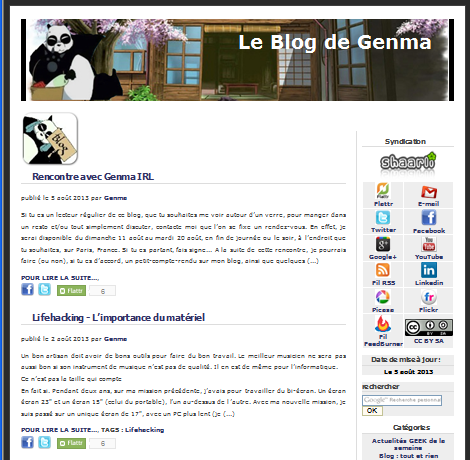
\includegraphics[scale=0.40] {./images/blog.png} 
\end{columns}
\end{frame}

\begin{frame}
\Huge{\centerline{Le BigData, ce sont toutes}}
\Huge{\centerline{ces données qui sont cumulées...}}
\end{frame}

\begin{frame}
\Huge{\centerline{Toutes ces traces qu'on laisse}}
\Huge{\centerline{sur Internet... sans le savoir}}
\end{frame}

%----------------------------------------------------------------------------------------
\begin{frame}
\begin{center}
\Huge{Toutes ces informations \\ que l'on donne... }
\end{center}
\end{frame}

%----------------------------------------------------------------------------------------
\begin{frame}
\frametitle{Diffusion de photos et autres selfies...}
\begin{center}

\includegraphics[scale=0.5] {./images/Leak02.png} 
\end{center}
\end{frame}

%----------------------------------------------------------------------------------------
\begin{frame}
\begin{center}
\Huge{Toutes ces informations \\ que l'on donne... }
\Huge{volontairement...\\~\\ou pas!}
\end{center}
\end{frame}

%----------------------------------------------------------------------------------------
\begin{frame}
\begin{center}
\Huge{Les données qui sont prises à notre insu}
\end{center}
\end{frame}

\begin{frame}
\begin{center}
\Huge{Comment est-on suivi à la trace sur Internet?}
\end{center}
\end{frame}

\begin{frame}
\frametitle{Comment est-on pisté ?}
\justifying{
\begin{block}{Toutes les publicités nous espionnent}
\begin{itemize}
\item Le bouton Like de Facebook : il permet à FaceBook de savoir que vous avez visité ce site, même si vous n'avez pas cliqué sur ce bouton.
\item Même si vous vous êtes correctement déconnecté de Facebook.
\item De même pour le bouton le +1 de Google, les scripts de Google Analytics, 
\item Toutes les publicités, Amazon...
\end{itemize}
\end{block}
}
\begin{center}

\includegraphics[scale=0.3] {./images/Facebook_like.png}
\end{center}
\end{frame}

%----------------------------------------------------------------------------------------
\begin{frame}
\frametitle{Les données qui sont prises à notre insu}
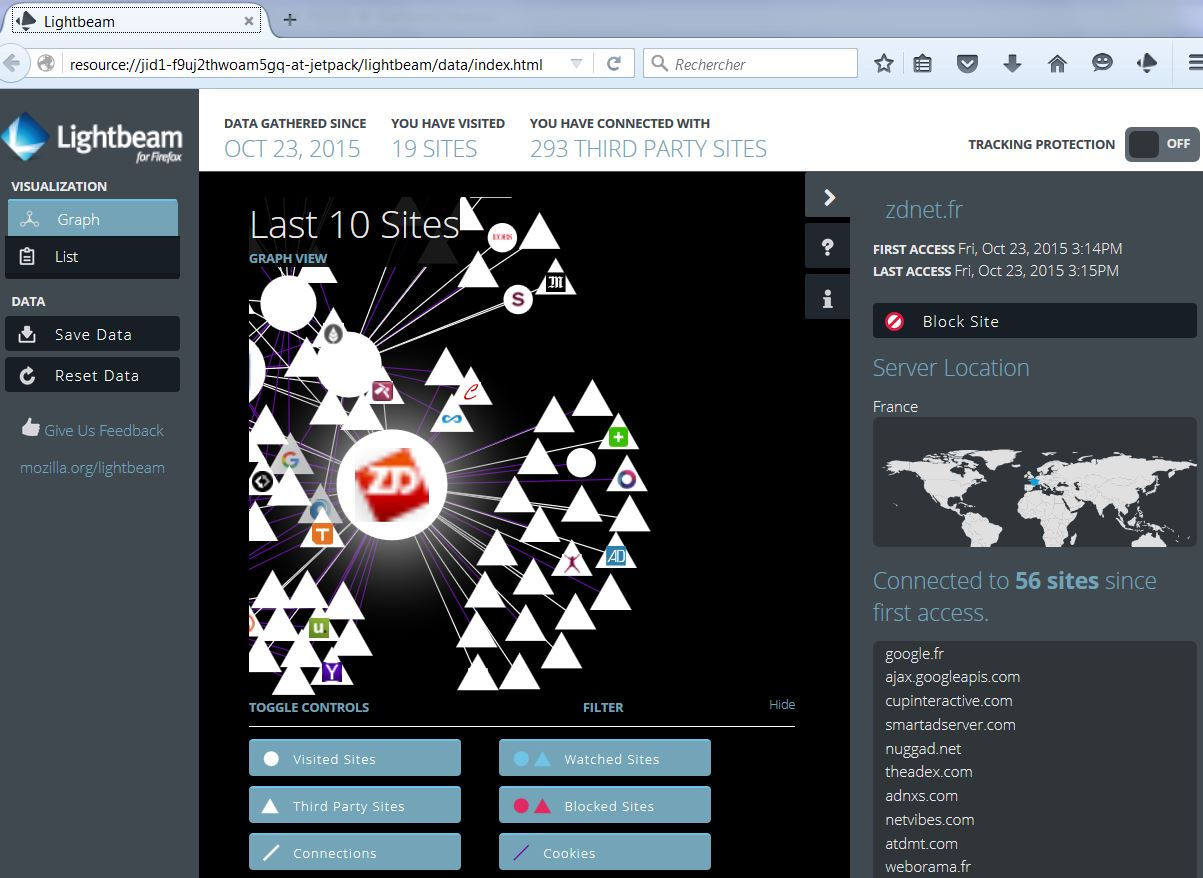
\includegraphics[scale=0.45] {./images/Lightbeam.jpg} 
\end{frame}

%----------------------------------------------------------------------------------------
\begin{frame}
\frametitle{Cloud - l'informatique dans les nuages}
\begin{block}{Définition du cloud}
\justifying{
\begin{itemize}
\item Le \emph{Cloud} , c'est l'ordinateur d'un autre.
\end{itemize}
}
\begin{center}

\includegraphics[scale=0.5] {./images/cloud.png} 
\end{center}
\end{block}
\end{frame}
%----------------------------------------------------------------------------------------

\begin{frame}
\begin{center}
\Huge{Les GAFAMs}\\~\\
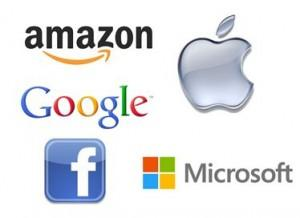
\includegraphics[scale=0.5] {./images/gafam.jpg} 
\end{center}
\end{frame}

%----------------------------------------------------------------------------------------
\begin{frame}
\frametitle{Les GAFAM}
\begin{block}{GAFAM : Google, Apple, Facebook, Amazon, Microsoft}
\begin{itemize}
\justifying{
\item Concentration des acteurs d’Internet autour de silos ;
\item Une centralisation nuisible (frein à l'innovation) ;
\item Les utilisateurs de ces services ne contrôlent plus leur vie numérique.
}
\end{itemize}
\end{block}
\end{frame}

%------------------------------------------------
\begin{frame}
\frametitle{GoogleFlu et Google trends}
\begin{block}{Présentation de Google Flux sur leur site}
\begin{itemize}
\justifying{
\item Nous avons remarqué que certains termes de recherche étaient des indicateurs efficaces de la propagation de la grippe. Google Flu rassemble donc des données de recherche Google pour fournir une estimation quasiment en temps réel de cette propagation à l'échelle mondiale. \url{http://www.google.org/flutrends/}
\item On peut aussi voir les recherches temps réels, par mot-clef, pays... \url{https://www.google.com/trends/}
}
\end{itemize}
\end{block}
\justifying{
Tout cela ne me laisse pas indifférent quand à \textbf{ la puissance de Google}. Et vous?
}
\end{frame}

%------------------------------------------------
\begin{frame}
\frametitle{Une carte de géolocalisation des photos de chat 1/2}
\justifying{
Un artiste s'est amusé à récupérer toutes les photos de chats qu'il trouvait sur le Web et en se basant sur les données de géolocalisation de ces photos, puis il a placé celles-ci sur une carte du monde. Voici ce que ça a donné :
}
\begin{center}
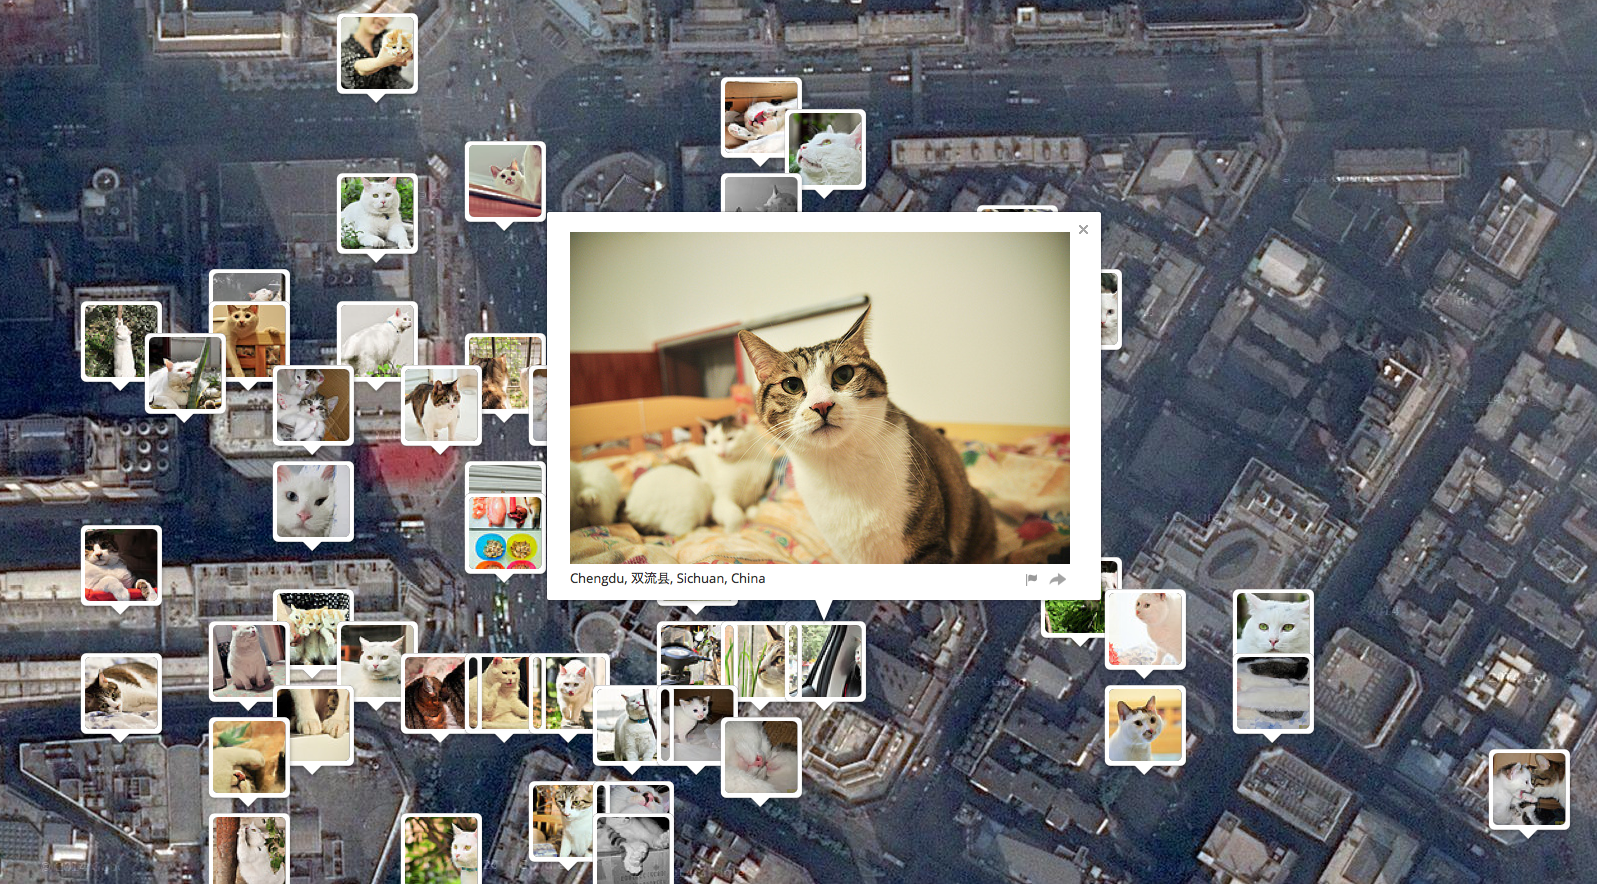
\includegraphics[scale=0.3]{./images/Chat_geolocalisaion.png}
\end{center}
\end{frame}
%------------------------------------------------
\begin{frame}
\frametitle{Une carte de géolocalisation des photos de chat 2/2}
On sait donc quel chat habite où - qui a un chat.
\\~\\
Réfléchissez-y. \textbf{Et si quelqu'un fasait la même chose mais avec d'autres photos...}
\end{frame}

%----------------------------------------------------------------------------------------
\begin{frame}
\begin{center}
\Huge{Sur Internet, si c'est gratuit, c'est VOUS le produit}
\end{center}
\end{frame}

%----------------------------------------------------------------------------------------
\begin{frame}
\begin{center}
\Huge{Big Data : comment s'en sortir ?}
\end{center}
\end{frame}

%----------------------------------------------------------------------------------------
\begin{frame}
\frametitle{4 piliers}
\begin{itemize}
\justifying{
\item Education
\item Logiciel libre
\item Décentralisation
\item Chiffrement de bout en bout
}
\end{itemize}
\end{frame}
%========================================================================================
\begin{frame}
\begin{center}
\Huge {Education}
\end{center}
\end{frame}

\begin{frame}
\begin{center}
\Huge{Comment se protéger ?\\ Un peu d'hygiène numérique}
\\~\\
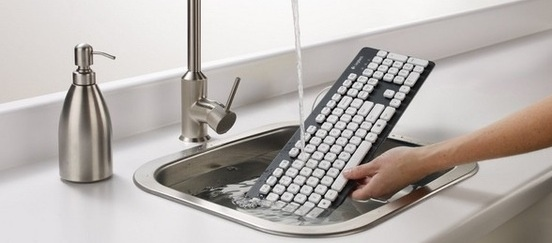
\includegraphics[scale=0.5]{./images/nettoyer_son_clavier.jpg}
\end{center}
\end{frame}

%----------------------------------------------------------------------------------------
\begin{frame}
\frametitle{L'hygiène numérique?}
\begin{block}{Une définition?}
\justifying{
L'hygiène est un ensemble de mesures destinées à prévenir les infections et l'apparition de maladies infectieuses.
\\~\\
L'hygiène numérique, ce sont des règles destinées à mieux utiliser son ordinateur, en sécurité, de façon simple.
}
\end{block}
\end{frame}

%----------------------------------------------------------------------------------------
\begin{frame}
\begin{center}
\Huge{Changer de moteur de recherche}
\\~\\

\includegraphics[scale=2] {./images/dontbeevil.jpg}
\end{center}
\end{frame}
%----------------------------------------------------------------------------------------
\begin{frame}
\begin{center}
\frametitle{Duckduckgo - Google tracks you. We don't.}

\url{https://duckduckgo.com}
\\~\\
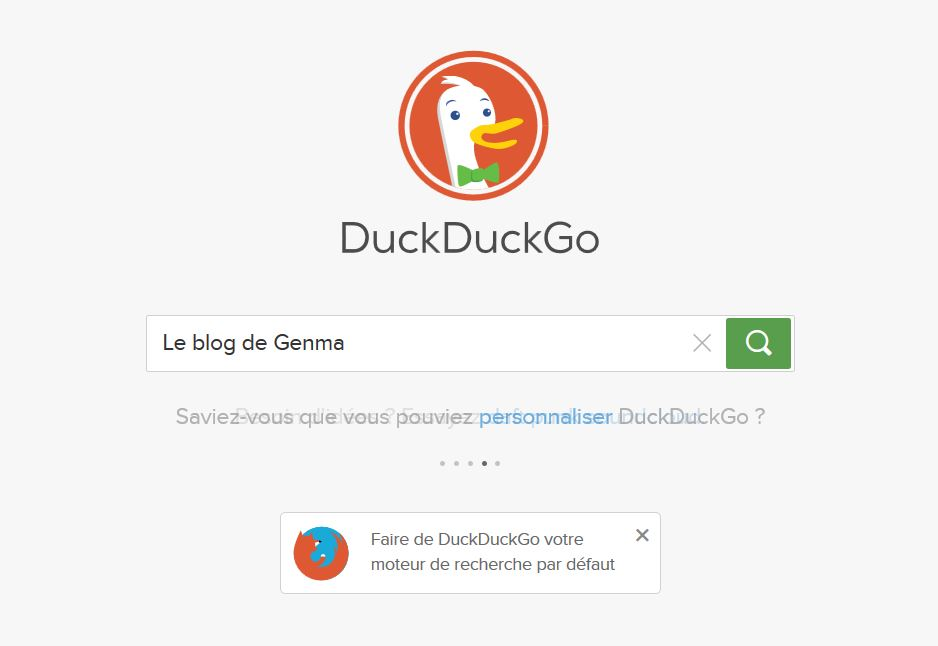
\includegraphics[scale=0.6] {./images/DuckDuckGo.jpg}
\end{center}
\end{frame}

\begin{frame}
\begin{center}
\frametitle{Par Framasoft}

Framabee \url{https://framabee.org} \\ou TontonRoger \url{https://tontonroger.org/}
\\~\\
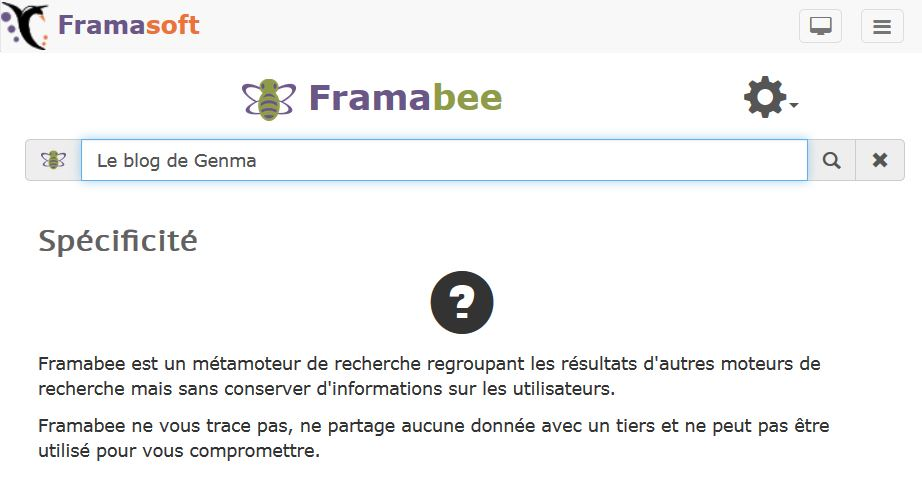
\includegraphics[scale=0.6] {./images/Framabee.jpg}
\end{center}
\end{frame}

\begin{frame}
\begin{center}
\frametitle{Qwant}

\url{https://qwant.com}
\\~\\

\includegraphics[scale=0.6] {./images/Qwant.jpg}
\end{center}
\end{frame}

%==================================================================================
\begin{frame}
\begin{center}
\Huge {Logiciel libre
\\ \emph{Open-source}
}
\end{center}
\end{frame}

%----------------------------------------------------------------------------------------
\begin{frame}
\begin{center}
\Huge{Navigateur}\\~\\Mozilla Firefox\\~\\

\includegraphics[scale=0.3] {./images/firefox.jpg}
\end{center}
\end{frame}

%----------------------------------------------------------------------------------------
\begin{frame}
\frametitle{Installer des extensions}
\begin{center}
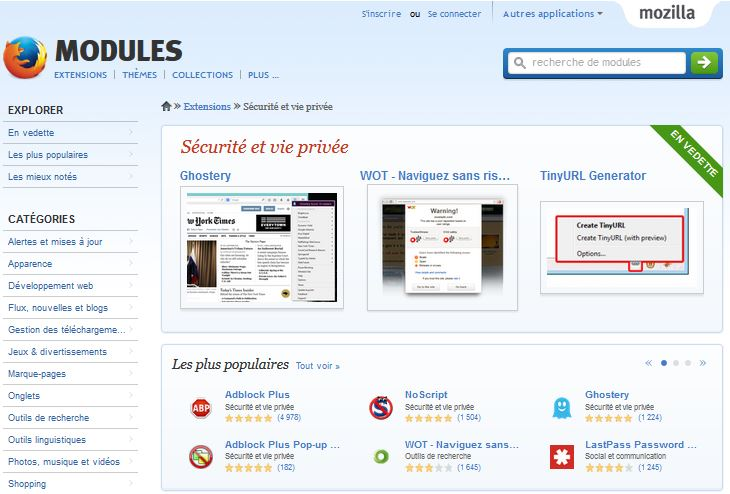
\includegraphics[scale=0.75] {./images/extensions_firefox.jpg}
\end{center}
\end{frame}

%----------------------------------------------------------------------------------------
\begin{frame}
\frametitle{Microblock - Bloquer les publicités}
\begin{center}
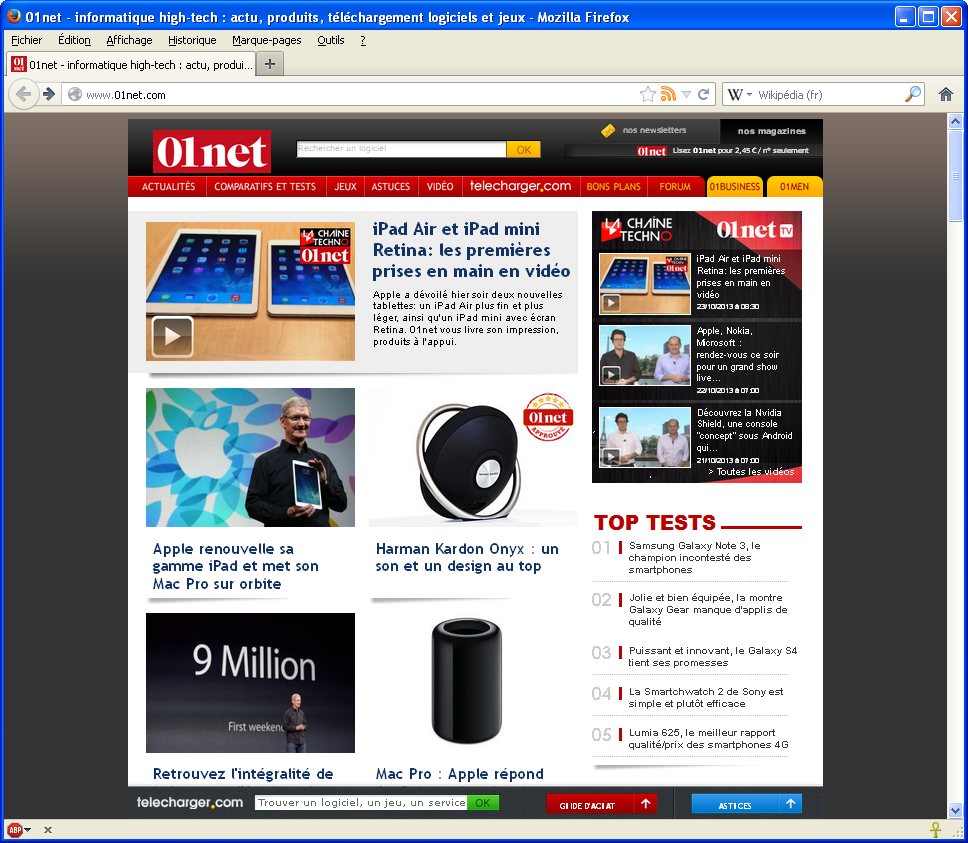
\includegraphics[scale=0.4] {./images/Adblock02.png}
\end{center}
\end{frame}

%----------------------------------------------------------------------------------------
\begin{frame}
\frametitle{Ghostery, Privacy Badger, Noscript...}
Bloque tous les trackers associés au site.
\begin{center}
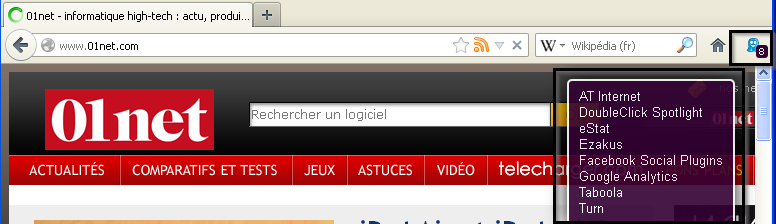
\includegraphics[scale=0.4] {./images/Ghostery_tracker.png}
\end{center}
\end{frame}

%========================================================================================
\begin{frame}
\begin{center}
\Huge {Décentralisation}
\end{center}
\end{frame}

\begin{frame}
\frametitle{Différents identités}
\begin{block}{Le pseudonyme, une forme de décentralisation de son identité}
\justifying{
\begin{itemize}
\justifying{
\item Quelles sont les données et informations que j'estime personnelles - confidentielles? 
\item Qu'est ce que je suis prêt-e à apprendre et à faire pour les protéger?
\item Usage d'un pseudonyme...
}
\end{itemize}
}\end{block}
\begin{center}

\includegraphics[scale=0.4]{./images/bannierepseudonymat.jpg}
\end{center}
\end{frame}

%----------------------------------------------------------------------------------------
\begin{frame}
\begin{center}
\frametitle{Framasoft et tous ses outils de Degooglisons}
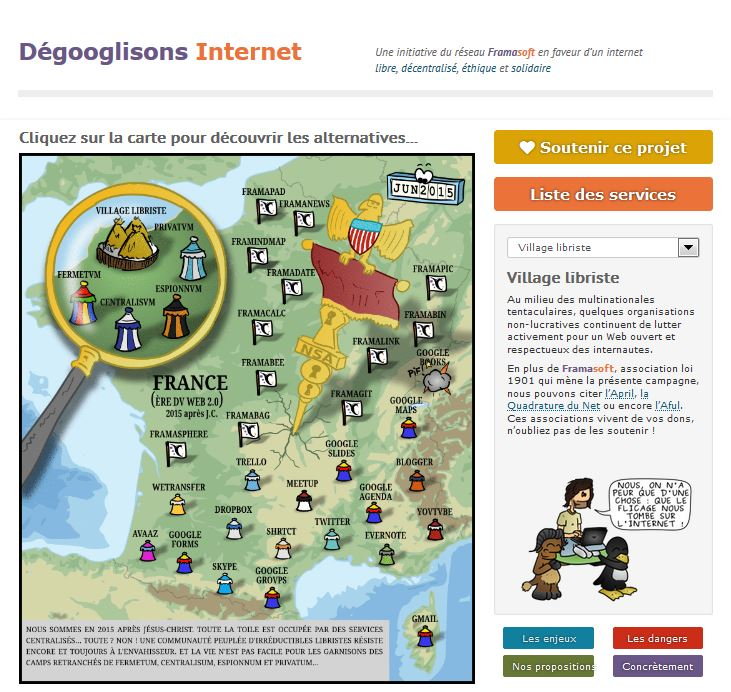
\includegraphics[scale=0.6] {./images/framasoft_degogglisons.jpg}
\end{center}
\end{frame}

%----------------------------------------------------------------------------------------
\begin{frame}
\Huge{\centerline{CHATONS}}
\begin{center}
\includegraphics[scale=0.5]{./images/Cute-Kittens-In-Computer-Case.jpg}
\end{center}
\end{frame}
%------------------------------------------------

%------------------------------------------------
\begin{frame}
\frametitle{CHATONS, le collectif anti-GAFAM ?}
Collectif d'Hébergeurs Alternatifs Transparents, Ouverts, Neutres et Solidaires \url{http://chatons.org/}

\begin{block}{Le projet \emph{Dégooglisons Internet} }
Consiste à proposer des services alternatifs face à un maximum de services que nous évaluons comme menaçants pour nos vies numériques.
\justifying{
\begin{itemize}
\item Rassembler
\item  Mutualiser
\item  Décentraliser
\item Donner de la visibilité
\item Fédérer
\item  Essaimer
\item Partager
\end{itemize}
}
\end{block}
Plus de détail sur \url{http://framablog.org/2016/02/09/chatons-le-collectif-anti-gafam/}

\end{frame}


%----------------------------------------------------------------------------------------
\begin{frame}
\begin{center}
\Huge{Changer de cloud}
\\~\\
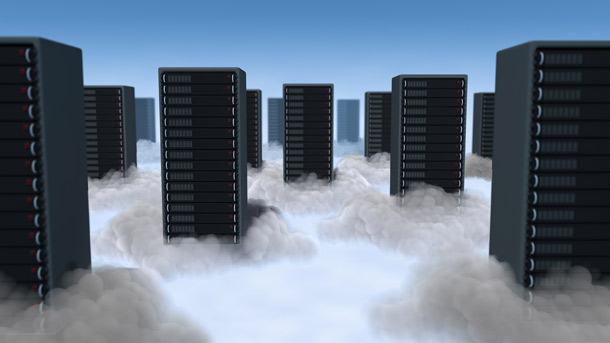
\includegraphics[scale=0.5] {./images/cloud_data_center.jpg}
\end{center}
\end{frame}

%----------------------------------------------------------------------------------------
\begin{frame}
\begin{center}
\frametitle{Cozycloud}
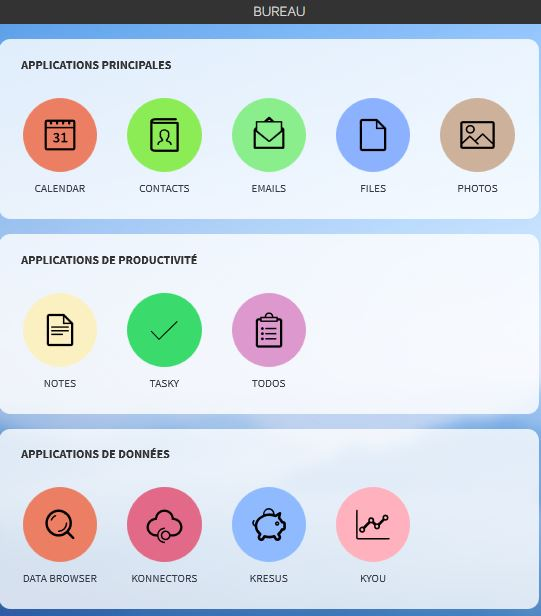
\includegraphics[scale=0.6] {./images/Cozycloud.jpg}
\end{center}
\end{frame}

%----------------------------------------------------------------------------------------
\begin{frame}
\begin{center}
\frametitle{Owncloud}
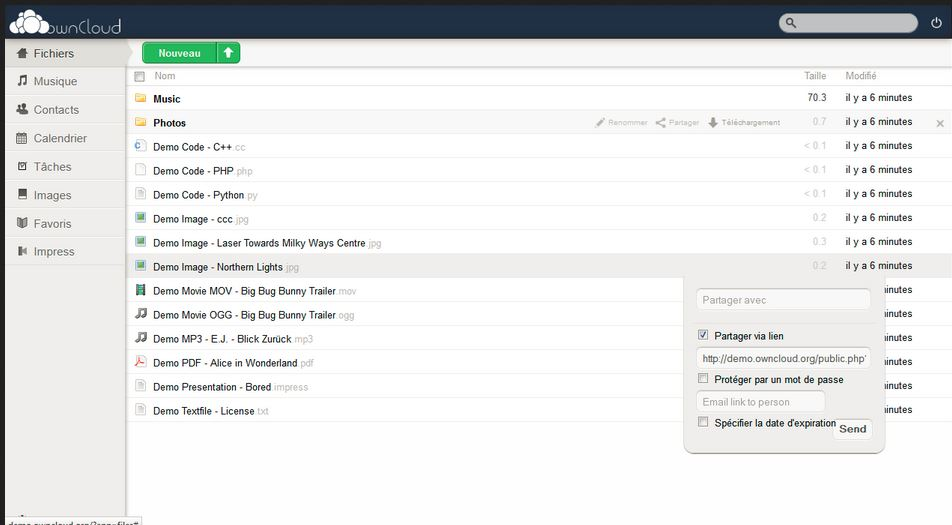
\includegraphics[scale=0.6] {./images/owncloud.jpg}
\end{center}
\end{frame}

%----------------------------------------------------------------------------------------
\begin{frame}
\begin{center}
\frametitle{La brique Internet}
\url{http://labriqueinter.net}
\\~\\
\includegraphics[scale=0.1] {./images/labriqueinternet.png}
\end{center}
\end{frame}

%========================================================================================
\begin{frame}
\begin{center}
\Huge {Chiffrement de bout en bout}
\end{center}
\end{frame}

%----------------------------------------------------------------------------------------
\begin{frame}
\begin{center}
\frametitle{Https}

\includegraphics[scale=0.5] {./images/https-everywhere.jpg}
\end{center}

\begin{block}{Un des intérêts du cadenas}
\justifying{
\justifying{
On sait quel site je regarde, Wikipédia par exemple, mais "on" ne sait pas quelle page je consulte (Wikipédia le sait).
\\~\\
Les informations circulent en \emph{cryptées}
}
}\end{block}
\end{frame}

\begin{frame}
\includegraphics[scale=0.25] {./images/DonnesCrypees.jpg}
\end{frame}
%----------------------------------------------------------------------------------------
\begin{frame}
\begin{center}
\Huge{Tor ? }
\\~\\ 
\includegraphics[scale=0.4]{./images/logo_tor.jpg}
\end{center}
\end{frame}

%----------------------------------------------------------------------------------------
\begin{frame}
\begin{center}
\Huge{Café vie privée, chiffrofête, cryptoparty}
\\~\\

\includegraphics[scale=0.3] {./images/LogoCafeViePrivee.jpg}
\end{center}
\end{frame}

\begin{frame}
\frametitle{Sorti du Big data...}
\begin{block}{4 piliers pour s'en sortir}
\begin{itemize}
\justifying{
\item Education
\item Logiciel libre
\item Décentralisation
\item Chiffrement de bout en bout
}
\end{itemize}
\end{block}
\end{frame}

%----------------------------------------------------------------------------------------
\begin{frame}
\frametitle{
\includegraphics[scale=0.4]{./images/Genma.jpg} \ \ \  Me contacter?}
\Huge{\centerline{Le Blog de Genma}}
\Huge{\centerline{http://genma.free.fr}}
\Huge{\centerline{~}}
\Huge{\centerline{Twitter : @genma}}
\end{frame}

%----------------------------------------------------------------------------------------
\begin{frame}
\begin{center}
\Huge{Merci de votre attention}
\\
\Huge{Place aux questions.}
\\~\\
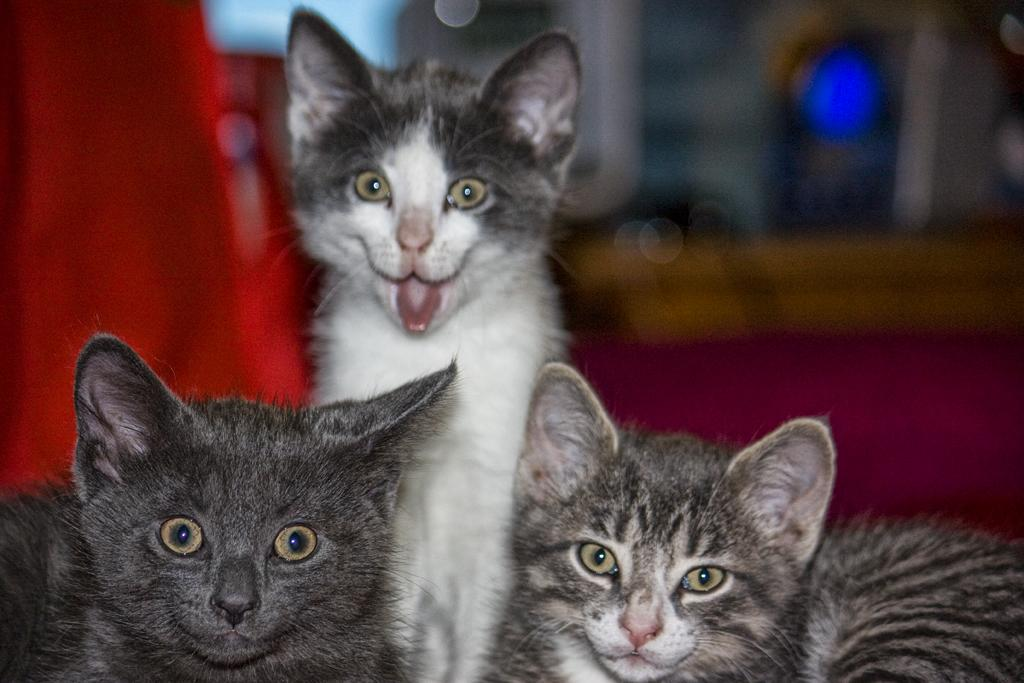
\includegraphics[scale=0.2] {./images/chat.jpg}
\end{center}
\end{frame}

%============================================================================================
\begin{frame}
\Huge{\centerline{ANNEXES}}
\end{frame}

%----------------------------------------------------------------------------------------
\begin{frame}
\frametitle{La navigation en mode privée 1/2}

\justifying{
\begin{block}{Quelles données ne sont pas enregistrées durant la navigation privée ?}
\begin{itemize}
\item pages visitées ;
\item saisies dans les formulaires et la barre de recherche ;
\item mots de passe ; 
\item liste des téléchargements ; 
\item cookies ;
\item fichiers temporaires ou tampons.
\end{itemize}
\end{block}
}
\end{frame}

%----------------------------------------------------------------------------------------
\begin{frame}
\frametitle{La navigation en mode privée 2/2}
\begin{center}
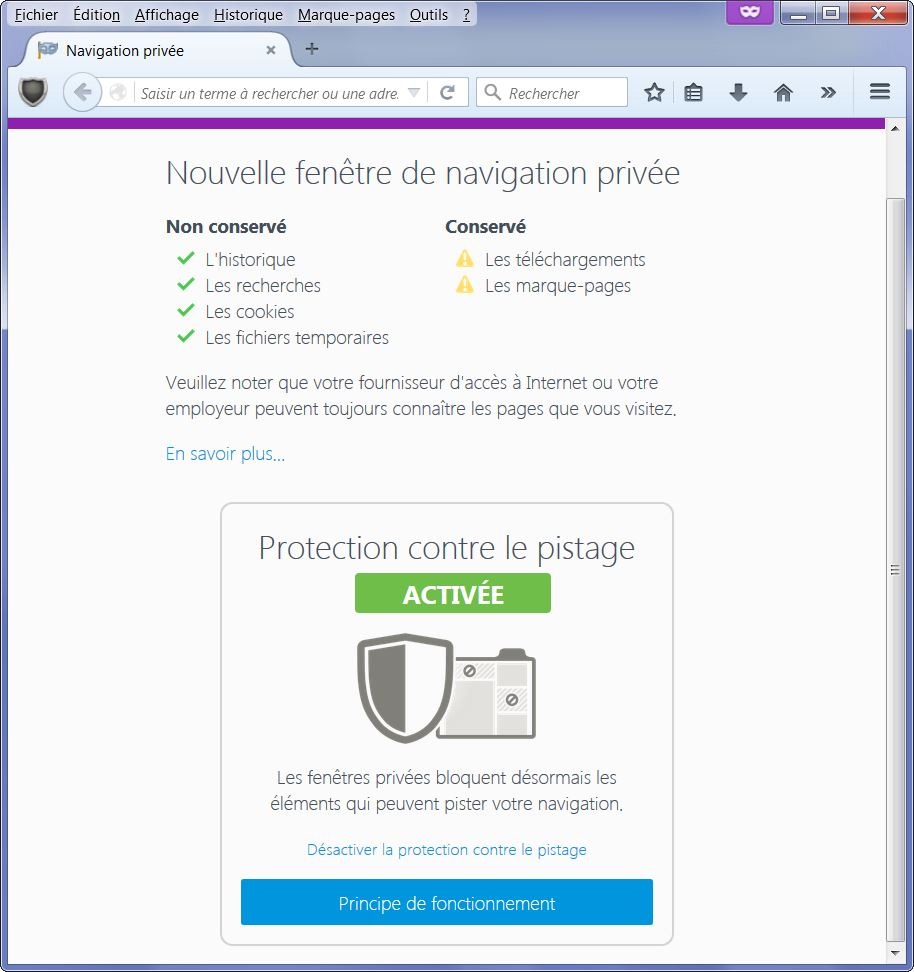
\includegraphics[scale=0.5] {./images/Navigation_privee.jpg} 
\end{center}
\end{frame}

\end{document}
